% Completa los datos convenientemente en las zonas marcadas con TODO

\documentclass{beamer}
%PARA VISUALIZAR PRESENTACIONN CON NOTAS USAR VISUALIZADOR "pdfpc":
%Para ver las notas, el cronometro y siguente diapo:
% pdfpc --notes=right slides.pdf
% "tecla p": para pausar el cronometro
\mode<presentation> {
  \usetheme{CambridgeUS}
  \usecolortheme{crane} % color naranja
}
\setbeamercolor{titlelike}{parent=structure,bg=yellow!85!orange} % Cambia el color de la caja del título de la página inicial

\setbeamertemplate{navigation symbols}{} % ocultar iconos de navegación
\setbeamerfont{subsection in toc}{size=\small} % reducir tamaño en TOC
\setbeamerfont{date}{size=\tiny}
\usepackage[spanish]{babel}
\usepackage[utf8]{inputenc}
\usepackage{graphicx}
\usepackage{booktabs}
\usepackage{hyperref}
\usepackage{multicol}
\usepackage{pgfpages}
\usepackage{listings}
\usepackage{multimedia}
\usepackage[export]{adjustbox}
\usepackage{outlines} % Para poner bullets tabulados (\1 \2 \3 ...) y no items

\usepackage{array,tabularx} % para tabular leyenda de ecuaciones
\newenvironment{conditions*} % entorno de "leyenda de ecuación"
  {\par\vspace{\abovedisplayskip}\noindent
   \tabularx{\columnwidth}{>{$}l<{$} @{\ : } >{\raggedright\arraybackslash}X}}
  {\endtabularx\par\vspace{\belowdisplayskip}}
  
% USO DE NOTAS
\setbeameroption{hide notes} % Para mostrar u ocultar (hide/show)
%\setbeameroption{show only notes} % Mostrar solo las notas
%\setbeameroption{show notes on second screen=right} % Mostrar notas en otra pantalla
\setbeamertemplate{note page}{ % asi solo muestro el texto de las notas
  \insertnote%
}

%========= TODO: datos internos del documento
\hypersetup{
	pdftitle={Defensa de trabajo de fin de grado de Pon tu nombre},
	pdfauthor={Pon tu nombre},
	pdfsubject={Pon aquí el título completo del trabajo},
	pdfkeywords={teaching, robotics, vision, sensors, actuators, raspberry},
	pdfproducer={pdfLaTeX},
  colorlinks=true,
  linkcolor=blue
}
%=========

%========= TODO: diapositiva de portada
\title[Sistema de detección de emociones]{Sistema de detección de emociones faciales mediante técnicas de Machine Learning adaptado a ROS para un robot de bajo coste basado en Raspberry Pi} % El título reducido aparece en la parte inferior de todas las diapositivas
                                         % El título completo aparece solo en la diapositiva de portada
\author[Javier Martínez Madruga]{Javier Martínez Madruga}
\institute[URJC]
{
\textit{\href{mailto:j.martinezma.2018@alumnos.urjc.es}{\color{blue}{\underline{j.martinezma.2018@alumnos.urjc.es}}}}\\
\vspace{0.5cm}
\includegraphics[width=3cm]{figs/logo-urjc}\\
\vspace{1cm}
Trabajo fin de grado
}
\date{28 de Junio de 2022}
%=========

%========= COMIENZO DEL DOCUMENTO
\begin{document}

%========= Portada inicial con notas
\begin{frame}[plain] % plain: quita header y footer
\large{\titlepage}
\note[item]{En esta presentación voy a hablar sobre...}
\note[item]{En primer lugar...}
\end{frame}

%========= Licencia
\begin{frame}
\input{licencia.tex}
\end{frame}

%========= Índice o tabla de contenidos (TOC)
\begin{frame}
\frametitle{Contenidos}
%\begin{multicols}{2} % si tengo muchas secciones, lo parte en dos columnas
  \tableofcontents[hideallsubsections] % no muestra subsecciones
%\end{multicols}
\note[item]{La presentaci\'on esta dividida en cuatro partes.}
\end{frame}

%========= Diapositiva "vacía" de comienzo de sección:
\section*{}
\begin{frame}{}
  \centering \Huge
  \emph{Introducción}
\note[item]{Comencemos con la introducción.}
\end{frame}

\section{Introducción}
%=========================================================
\begin{frame}
\frametitle{Robótica de Servicio y HRI}

\begin{figure}
  \begin{center}
    \subfigure{\includegraphics[width=33mm]{figs/roomba.png}}
    \subfigure{\includegraphics[width=35mm]{figs/spot.jpg}}
    \subfigure{\includegraphics[width=46mm]{figs/waymo.jpg}}
  \end{center}
\end{figure}
\begin{figure}
  \begin{center}
    \subfigure{\includegraphics[width=39mm]{figs/mako.png}}
    \subfigure{\includegraphics[width=55mm]{figs/robin.png}}
  \end{center}
\end{figure}

\end{frame}

%=============================================================
\begin{frame}
\frametitle{Visión Artificial y Machine Learning}
\begin{figure}
    \centering
    \includegraphics[width=9cm]{figs/Apps-de-reconocimiento-facial-1.jpg}
\end{figure}
    
\end{frame}

%=============================================================
\begin{frame}
\frametitle{Sistemas empotrados}
\begin{figure}
    \centering
    \includegraphics[width=10cm]{figs/raspberry_en_mano_rojo.png}
\end{figure}
    
\end{frame}

%========= Diapositiva con ítems resaltados con colores:
% \begin{frame}
% \frametitle{Situación de la Robótica}
% \begin{itemize}
% \item La \textcolor{red}{tecnología} está cada vez más presente en la vida cotidiana.
% \item Los robots de servicio aparecen en el \textcolor{blue}{mercado}.
% \item La \textcolor{red}{domótica} presenta cada vez más aplicaciones domésticas.
% \end{itemize}
% \end{frame}

% \subsection{Contexto específico}
% %========= Diapositiva con bloques:
% \begin{frame}
% \frametitle{Precedentes de la robótica}
% \begin{block}{Primera revolución industrial de 1800}
% Productos fabricados por \textcolor{blue}{máquinas}. La \textcolor{red}{máquina de vapor} fue clave.
% \end{block}
% \end{frame}

%========= Diapositiva con bullets en diferentes niveles (outline):
% \section{Principios de transducción}
% \subsection{Principio de transducción piezoresistivo}
% \begin{frame}
% \frametitle{Conceptos}
% \begin{outline}
% \1 Piezoresistividad: relación entre resistencia eléctrica y deformación.
% \2 Material piezoresistivo: (1) material en reposo (átomos en equilibrio).
% \3 (2) Si sufre deformación, movimiento átomos, modifican su resistividad.
% \2 Resistencia vs. resistividad de un material.
% \3 Resistencia: depende del volumen del material a tratar.
% \3 Resistividad: caract. intrínseca relacionada con colocación de átomos.
% \end{outline}
% \end{frame}

\section*{}
\begin{frame}{}
  \centering \Huge
  \emph{Objetivos}
\note[item]{Pasemos ahora a comentar los objetivos que nos hemos con este trabajo.}
\end{frame}

\section{Objetivos}
\begin{frame}
\frametitle{Descripción del problema}
\begin{block}{Objetivo principal}
Desarrollar una herramienta de \textbf{reconocimiento de emociones faciales} capaz de funcionar en un sistema robótico de \textbf{bajo coste}.
\end{block}
\begin{block}{Subobjetivos}
\begin{itemize}
\item Estudiar el estado del arte.
\item Optimizar y adaptar la técnica escogida.
\item Generar un dataset de valor.
\item Entrenar un modelo con varios clasificadores.
\item Integrar la herramienta en ROS.
\end{itemize}
\end{block}
\end{frame}

\begin{frame}
\frametitle{Metodología}
\begin{figure}
    \centering
    \includegraphics[width=10cm]{figs/metodologia.png}
\end{figure}
\end{frame}

\section*{}
\begin{frame}{}
  \centering \Huge
  \emph{Plataforma de desarrollo}
\note[item]{Una vez descritos los objetivos, veamos qué hemos hecho para alcanzarlos.}
\end{frame}

\section{Plataforma de desarrollo}
\begin{frame}
\frametitle{Raspberry}
\begin{figure}
    \centering
    \includegraphics[width=6cm]{figs/pi-camera-attached.jpg}
\end{figure}
\begin{figure}
    \centering
    \includegraphics[width=6cm]{figs/Raspberry_Pi_OS_Logo.png}
\end{figure}
\end{frame}

\begin{frame}{Herramientas Software}
\begin{figure}
    \centering
    \includegraphics[width=8.5cm]{figs/herramientas_software.png}
\end{figure}
\end{frame}

\begin{frame}{Algoritmos de Machine Learning}
\begin{figure}
    \begin{center}
        \includegraphics[width=10cm]{figs/algoritmosML.png}
    \end{center}
\end{figure}
\end{frame}

\section*{}
\begin{frame}{}
  \centering \Huge
  \emph{Sistema de detección de emociones}
\note[item]{Una vez descritos los objetivos, veamos qué hemos hecho para alcanzarlos.}
\end{frame}

\section{Sistema de detección de emociones}
\begin{frame}{Esquema general}
\begin{figure}
    \begin{center}
        \includegraphics[width=12cm]{figs/metodo_sin_secciones.png}
    \end{center}
\end{figure}
\end{frame}

\subsection{Detección de puntos faciales}
\begin{frame}{MediaPipe FaceMesh}
\begin{figure}
  \begin{center}
    \subfigure{\includegraphics[width=48mm]{figs/mediapipe_buena_luz.png}}
    \subfigure{\includegraphics[width=60mm]{figs/canonical_face_model_uv_visualization.png}}
  \end{center}
\end{figure}
\end{frame}

\subsection{Extracción de información}
\begin{frame}{Malla emocional}
\begin{figure}
    \begin{center}
        \includegraphics[width=7cm]{figs/emotional_mesh.png}
    \end{center}
\end{figure}
\end{frame}

\begin{frame}{FACS y EMFACS}
\begin{table}[h!]
\begin{minipage}{0.45\linewidth}
\centering
\begin{adjustbox}{max width=\textwidth}
\begin{tabular}{|c|c|}
     \hline
    \textbf{AU} & \textbf{Descripciones FACS} \\
    \hline
     1 & Interior de las cejas elevado\\ 
     2 & Exterior de las cejas elevado \\ 
     4 & Cejas bajadas \\
     5 & Párpado superior elevado\\
     6 & Mejillas elevadas \\ 
     7 & Párpados tensos \\
     9 & Nariz arrugada \\
     10 & Labio superior elevado \\
     12 & Comisuras de los labios elevados \\ 
     15 & Comisuras de los labios hacia abajo \\
     16 & Labio inferior hacia abajo \\
     17 & Barbilla elevada \\
     20 & Labios apretados y estirados\\
     22 & Labios en forma de \textit{o} \\
     23 & Labios tensos \\
     24 & Labios presionados \\
     25 & Labios separados \\
     26 & Boca abierta (mandíbula caída)\\
     27 & Boca abierta \\
     \hline
 \end{tabular}
\end{adjustbox}
\end{minipage} \hspace{0.1cm}
\begin{minipage}{0.45\linewidth}
\centering
\begin{adjustbox}{max width=\textwidth}
\begin{tabular}{|c|c|}
     \hline
    \textbf{Emoción} & \textbf{AU} \\
    \hline
     Felicidad & 6 + 12\\ 
     Tristeza & 1 + 4 + 15 \\ 
     Sorpresa & 1 + 2 + 5 + 26 \\
     Miedo & 1 + 2 + 4 + 5 + 7 + 20 + 26\\
     Enfado & 4 + 5 + 7 + 23 \\ 
     Asco & 9 + 15 + 17 \\
     Desprecio & 12 + 14 \\
     \hline
 \end{tabular}
\end{adjustbox}
\end{minipage}
\end{table}
\end{frame}

\subsection{Generación del dataset}
\begin{frame}{The Extended Cohn-Kanade Dataset
(CK+)}
\begin{figure}[h!]
  \begin{center}
    \subcapcentertrue
    \subfigure{\includegraphics[width=3.5cm]{figs/sujeto_triste.png}}
    \subfigure{\includegraphics[width=3.5cm]{figs/sujeto_feliz.png}}
    \subfigure{\includegraphics[width=3.5cm]{figs/sujeto_sorprendido.png}}
  \end{center}
\end{figure}
\begin{block}{Contenido}
\begin{itemize}
    \item 327 imágenes etiquetadas
    \item 7 clases (anger, contempt, disgust, fear, happy, sadness, surprise)
\end{itemize}
\end{block}
\end{frame}

\begin{frame}{Dataset generado}
\begin{table}
\begin{center}
\begin{adjustbox}{max width=250}
\begin{tabular}{|c|c|c|c|c|c|c|}
     \hline
    \textbf{X0} & \textbf{X1} & \textbf{X2} & \textbf{...} & \textbf{X19} & \textbf{X20} & \textbf{y}\\
    \hline
    54.288044 & 37.570711 & 154.655589 & ... & 44.625203 & 63.887010 & 1.0\\ 
    44.670597 & 35.229102 & 148.630240 & ... & 47.334403 & 61.278073 & 1.0\\
    46.613914 & 36.808837 & 161.148375 & ... & 57.291823 & 64.390395 & 1.0\\
    49.404349 & 47.407905 & 153.817836 & ... & 49.880184 & 61.894869 & 1.0\\
    42.510847 & 43.626048 & 146.891826 & ... & 46.965439 & 59.971707 & 1.0\\
    ... & ... & ... & ... & ... & ... & ...\\
    23.444336 & 97.667648 & 88.384186 & ... & 28.011004 & 63.905389 & 7.0\\
    24.634940 & 96.406625 & 93.413763 & ... & 28.637606 & 63.551521 & 7.0\\
    22.425106 & 105.319774 & 87.727242 & ... & 30.811141 & 61.646881 & 7.0\\
    15.966920 & 120.968600 & 60.790043 & ... & 28.018767 & 56.442379 & 7.0\\
    19.667632 & 104.568158 & 80.332991 & ... & 29.088510 & 64.107810 & 7.0\\
     \hline
 \end{tabular}
 \end{adjustbox}
\end{center}
\end{table}
\begin{block}{Contenido}
\begin{itemize}
    \item 226 muestras
    \item 21 características
    \item 4 clases (anger, happy, sadness, surprise)
\end{itemize}
\end{block}
\end{frame}

\subsection{Entrenamiento del modelo}
\begin{frame}{Validación cruzada K-Fold Stratified de 4 pliegues}
\begin{figure}
    \begin{center}
        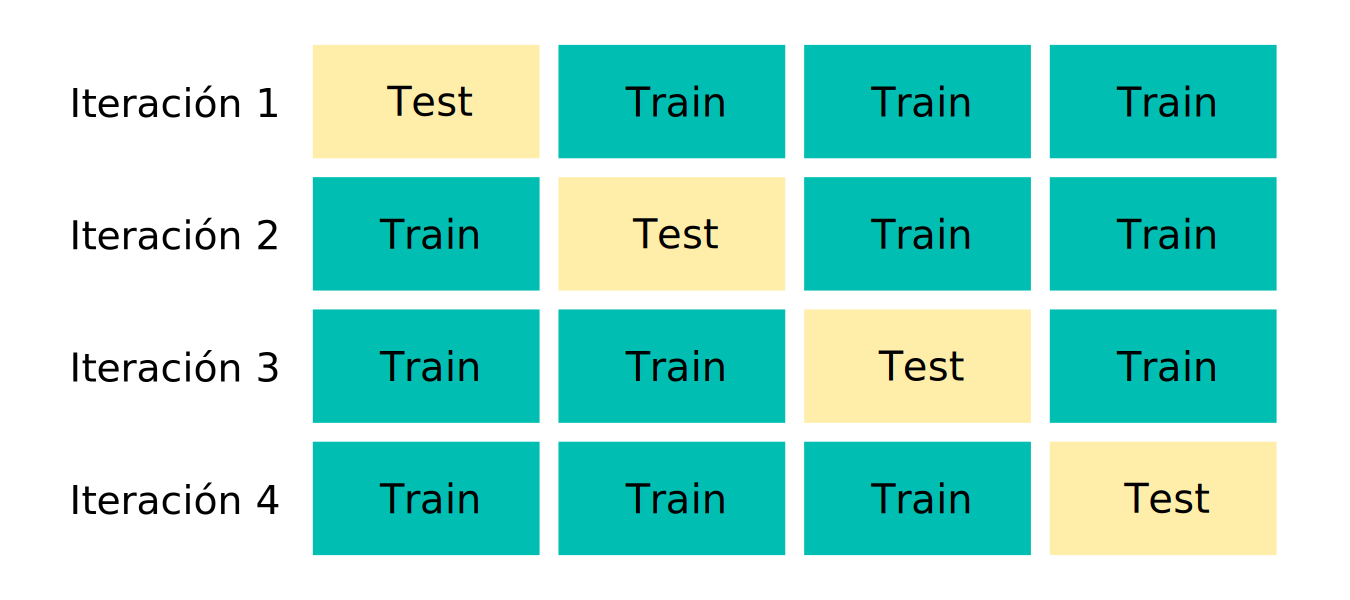
\includegraphics[width=12cm]{figs/KFold_explanation.png}
    \end{center}
\end{figure}
\end{frame}

\begin{frame}{Búsqueda de los parámetros óptimos}
    \begin{figure}
    \begin{center}
        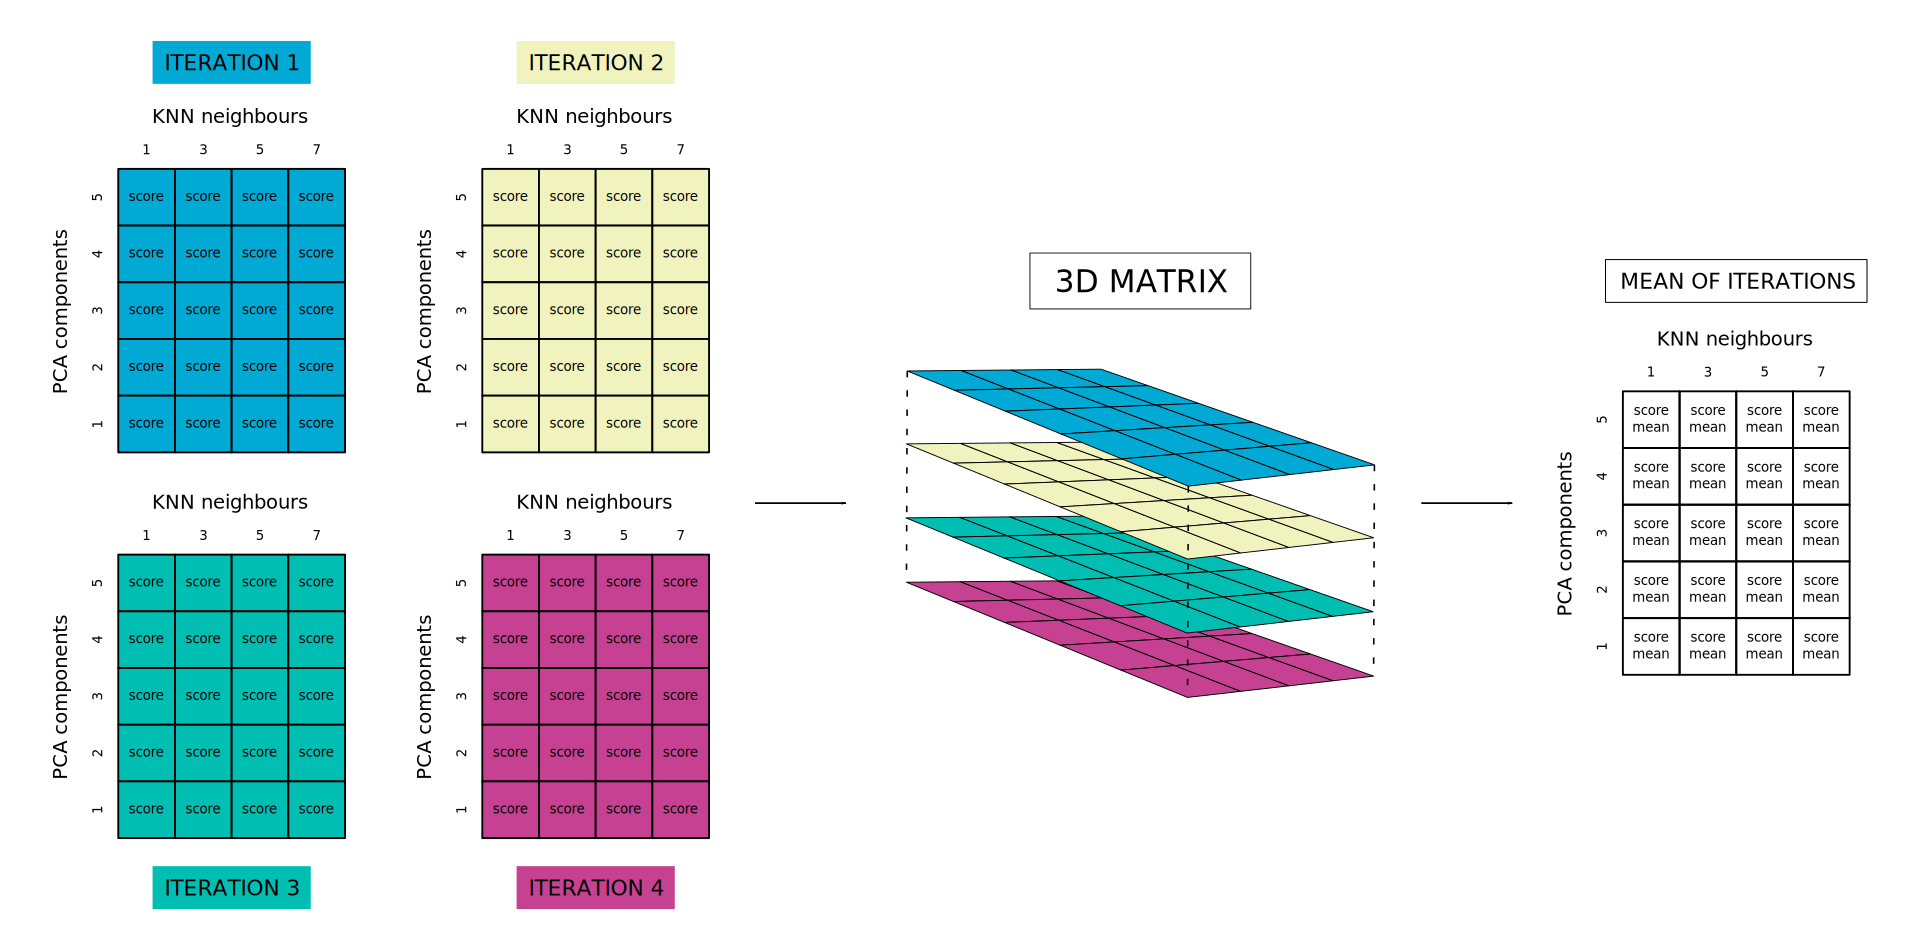
\includegraphics[width=12cm]{figs/KFold_KNN_PCA.png}
    \end{center}
\end{figure}
\end{frame}

\begin{frame}{Parámetros óptimos}
\begin{block}{Intervalos de valores testeados}
\begin{itemize}
    \item PCA: número de \textit{componentes} en [2, 20]
    \item KNN: valores impares de \textit{k} en [1, 13]
    \item SVM: valores de \textit{C} en [1, 999] con saltos de 10
    \item MLP: 1 capa oculta de [5, 24] \textit{neuronas}
\end{itemize}
\end{block}

\begin{table}[H]
\begin{center}
\begin{tabular}{|c|c|}
    \hline
    \textbf{Clasificador y PCA} & \textbf{Parámetros} \\
    \hline
     KNN y PCA & k = 7, n\_components = 11\\
     SVM y PCA & C = 21, n\_components = 11\\
     MLP y PCA & hidden\_layer\_sizes = (17), n\_components = 11\\
     \hline
 \end{tabular}
\end{center}
\end{table}
\end{frame}

\begin{frame}{Resultados del entrenamiento}
\begin{table}[H]
\begin{center}
\begin{tabular}{|c|c|c|c|c|}
     \hline
    \textbf{Clasificador} & \textbf{Accuracy} & \textbf{Precision} & \textbf{Recall} & \textbf{F1-score}\\
    \hline
     KNN & 0.95 & 0.93 & 0.94 & 0.92\\
     SVM & 0.95 & 0.93 & 0.92 & 0.92\\
     MLP & 0.95 & 0.95 & 0.93 & 0.93\\
     \hline
\end{tabular}
\end{center}
\end{table}
\end{frame}

\subsection{Funcionamiento del sistema}
\begin{frame}{Esquema de funcionamiento del sistema}
\begin{figure}
    \begin{center}
        \includegraphics[width=11cm]{figs/func.png}
    \end{center}
\end{figure}
\end{frame}

\subsection{Integración en ROS}
\begin{frame}{Esquema de funcionamiento del sistema en ROS}
\begin{figure}
    \begin{center}
        \includegraphics[width=12cm]{figs/paquete_ros.png}
    \end{center}
\end{figure}
\end{frame}

\begin{frame}{Parámetros de configuración}
\begin{figure}
  \centering
  \includegraphics[width=12cm]{figs/yamls.png}
\end{figure}
\end{frame}

\subsection{Uso y rendimiento}
\begin{frame}{Ejemplo de funcionamiento con 1 cara}
\begin{figure}[h!]
  \begin{center}
    \subcapcentertrue
    \subfigure{\includegraphics[width=45mm]{figs/prediccion_happy.png}}
    \subfigure{\includegraphics[width=45mm]{figs/prediccion_anger.png}}
    \subfigure{\includegraphics[width=45mm]{figs/prediccion_sadness.png}}
    \subfigure{\includegraphics[width=45mm]{figs/prediccion_surprise.png}}
  \end{center}
\end{figure}
\end{frame}

\begin{frame}{Ejemplo de funcionamiento con 2 caras}
\begin{figure}[h!]
  \begin{center}
    \subcapcentertrue
    \subfigure{\includegraphics[width=45mm]{figs/prediccion_happy_surprise.png}}
    \subfigure{\includegraphics[width=80mm]{figs/salida_topic.png}}
  \end{center}
\end{figure}
\end{frame}

\begin{frame}{Rendimiento}
\begin{block}{max\_num\_faces: 1}
\begin{table}[H]
\begin{center}
\begin{adjustbox}{max width=\textwidth}
\begin{tabular}{|c|c|c|c|}
     \hline
    \textbf{Caras detectadas} & \textbf{Media de FPS} & \textbf{Valor máximo de FPS} & \textbf{Valor mínimo de FPS}\\
    \hline
     1 & 13.18 & 15.13 & 11.04\\
     \hline
 \end{tabular}
 \end{adjustbox}
\end{center}
\end{table}
\end{block}

\begin{block}{max\_num\_faces: 2}
\begin{table}[H]
\begin{center}
\begin{adjustbox}{max width=\textwidth}
\begin{tabular}{|c|c|c|c|}
     \hline
    \textbf{Caras detectadas} & \textbf{Media de FPS} & \textbf{Valor máximo de FPS} & \textbf{Valor mínimo de FPS}\\
    \hline
     1 & 11.11 & 11.97 & 9.18\\
     2 & 7.53 & 8.35 & 6.96\\
     \hline
 \end{tabular}
 \end{adjustbox}
\end{center}
\end{table}
\end{block}

\begin{block}{max\_num\_faces: 3}
\begin{table}[H]
\begin{center}
\begin{adjustbox}{max width=\textwidth}
\begin{tabular}{|c|c|c|c|}
     \hline
    \textbf{Caras detectadas} & \textbf{Media de FPS} & \textbf{Valor máximo de FPS} & \textbf{Valor mínimo de FPS}\\
    \hline
     1 & 11.05 & 11.72 & 9.41\\
     2 & 6.77 & 7.61 & 6.15\\
     3 & 5.37 & 6.93 & 5.02\\
     \hline
 \end{tabular}
 \end{adjustbox}
\end{center}
\end{table}
\end{block}
\end{frame}

\section*{}
\begin{frame}{}
  \centering \Huge
  \emph{Estudios de optimización}
\note[item]{Para acabar esta presentación, vamos a repasar lo hecho, unas breves conclusiones y las líneas futuras.}
\end{frame}

\section{Estudios de optimización}
\subsection{Búsqueda del detector de puntos faciales óptimo}
\begin{frame}{Estudio de rendimiento para dlib y MediaPipe}
\begin{figure}[h!]
  \begin{center}
    \includegraphics[width=12cm]{figs/pruebas_rendimiento_puntos.png}
  \end{center}
\end{figure}
\end{frame}

\begin{frame}{Estudio de precisión para dlib y MediaPipe}
\begin{figure}[h!]
  \begin{center}
    \subcapcentertrue
    \subfigure{\includegraphics[width=25mm]{figs/dlib_buena_luz.png}}
    \subfigure{\includegraphics[width=25mm]{figs/dlib_mala_luz.png}}
    \subfigure{\includegraphics[width=25mm]{figs/dlib_cubiertos.png}}
    \subfigure{\includegraphics[width=25mm]{figs/dlib_girados.png}}
  \end{center}
\end{figure}

\begin{figure}[h!]
  \begin{center}
    \subcapcentertrue
    \subfigure{\includegraphics[width=25mm]{figs/mediapipe_buena_luz.png}}
    \subfigure{\includegraphics[width=26mm]{figs/mediapipe_mala_luz.png}}
    \subfigure{\includegraphics[width=25mm]{figs/mediapipe_cubiertos.png}}
    \subfigure{\includegraphics[width=25mm]{figs/mediapipe_girados.png}}
  \end{center}
\end{figure}
\end{frame}

\subsection{Cantidad de ángulos a utilizar en el dataset}
\begin{frame}{Estudio de ángulos más influyentes en cada emoción}
\begin{figure}[h!]
  \begin{center}
    \includegraphics[width=7cm]{figs/emotional_mesh_todos_angulos.png}
  \end{center}
\end{figure}
\end{frame}

\begin{frame}{Resultados del estudio de ángulos más influyentes}
\begin{figure}[h!]
  \begin{center}
    \subcapcentertrue
    \subfigure{\includegraphics[width=38mm]{figs/diferencia_happy.png}}
    \subfigure{\includegraphics[width=38mm]{figs/diferencia_sadness.png}}
    \subfigure{\includegraphics[width=38mm]{figs/diferencia_surprise.png}}
    \subfigure{\includegraphics[width=38mm]{figs/diferencia_fear.png}}
    \subfigure{\includegraphics[width=38mm]{figs/diferencia_anger.png}}
    \subfigure{\includegraphics[width=38mm]{figs/diferencia_disgust.png}}
  \end{center}
\end{figure}
\end{frame}

\begin{frame}{Resultados del estudio de ángulos más influyentes}
\begin{table}[H]
\begin{center}
\begin{tabular}{|c|c|}
     \hline
    \textbf{Emoción} & \textbf{Ángulos influyentes} \\
    \hline
     Felicidad & 4, 2, 18, 12, 8 \\
     Tristeza & 2, 1, 12, 16, 14 \\
     Sorpresa & 1, 2, 0, 4, 19 \\
     Miedo & 2, 4, 6, 1, 14 \\
     Enfado & 2, 12, 1, 16, 15 \\
     Asco & 12, 16, 2, 15, 1 \\
     Desprecio & 2, 1, 4, 0, 19 \\
     \hline
 \end{tabular}
\end{center}
\end{table}
\end{frame}

\begin{frame}{Estudio de simetría de las emociones}
\begin{figure}[h!]
  \begin{center}
    \includegraphics[width=7cm]{figs/emotional_mesh_2_mitades.png}
  \end{center}
\end{figure}
\end{frame}

\begin{frame}{Resultados del estudio de simetría}
\begin{figure}[h!]
  \begin{center}
    \subcapcentertrue
    \subfigure{\includegraphics[width=38mm]{figs/diferencia_izq_der_happy.png}}
    \subfigure{\includegraphics[width=38mm]{figs/diferencia_izq_der_sadness.png}}
    \subfigure{\includegraphics[width=38mm]{figs/diferencia_izq_der_surprise.png}}
    \subfigure{\includegraphics[width=38mm]{figs/diferencia_izq_der_fear.png}}
    \subfigure{\includegraphics[width=38mm]{figs/diferencia_izq_der_anger.png}}
    \subfigure{\includegraphics[width=38mm]{figs/diferencia_izq_der_disgust.png}}
  \end{center}
\end{figure}
\end{frame}

\subsection{Búsqueda del dataset óptimo para el entrenamiento}
\begin{frame}{Búsqueda del dataset con más rendimiento}
\begin{block}{Resultados entrenamiento dataset1}
\begin{table}[H]
\begin{center}
\begin{tabular}{|c|c|c|c|c|}
     \hline
    \textbf{Clasificador} & \textbf{Accuracy} & \textbf{Precision} & \textbf{Recall} & \textbf{F1-score}\\
    \hline
     KNN & 0.82 & 0.76 & 0.74 & 0.74\\
     SVM & 0.84 & 0.79 & 0.78 & 0.77\\
     MLP & 0.82 & 0.78 & 0.78 & 0.77\\
     \hline
 \end{tabular}
\end{center}
\end{table}
\end{block}

\begin{block}{Resultados entrenamiento dataset2}
\begin{table}[H]
\begin{center}
\begin{tabular}{|c|c|c|c|c|}
     \hline
    \textbf{Clasificador} & \textbf{Accuracy} & \textbf{Precision} & \textbf{Recall} & \textbf{F1-score}\\
    \hline
     KNN & 0.83 & 0.79 & 0.75 & 0.75\\
     SVM & 0.84 & 0.80 & 0.77 & 0.78\\
     MLP & 0.84 & 0.81 & 0.80 & 0.80\\
     \hline
 \end{tabular}
\end{center}
\end{table}
\end{block}
\end{frame}

\begin{frame}{Resultados del entrenamiento con SVM de cada iteración de K-Fold usando el dataset2}
    \begin{table}[h!]
\begin{minipage}{0.48\linewidth}
\centering
\begin{adjustbox}{max width=\textwidth}
\begin{tabular}{|c|c|c|c|}
\hline
\textbf{Clase} & \textbf{Precision} & \textbf{Recall} & \textbf{F1-score}\\
\hline
     Enfado & 0.67 & 0.50 & 0.57\\
     Desprecio & 0.67 & 0.50 & 0.57\\
     Asco & 0.76 & 0.87 & 0.81\\
     Miedo & 0.67 & 1.00 & 0.80\\
     Felicidad & 0.94 & 0.94 & 0.94\\
     Tristeza & 0.83 & 0.71 & 0.77\\
     Sorpresa & 0.95 & 0.95 & 0.95\\
\hline
\end{tabular}
\end{adjustbox}
\vspace{0.4cm}

\begin{adjustbox}{max width=\textwidth}
\begin{tabular}{|c|c|c|c|}
\hline
\textbf{Clase} & \textbf{Precision} & \textbf{Recall} & \textbf{F1-score}\\
\hline
     Enfado & 0.75 & 0.82 & 0.78\\
     Desprecio & 0.67 & 0.80 & 0.73\\
     Asco & 0.82 & 0.93 & 0.87\\
     Miedo & 0.80 & 0.67 & 0.73\\
     Felicidad & 0.94 & 0.94 & 0.94\\
     Tristeza & 1.00 & 0.57 & 0.73\\
     Sorpresa & 0.95 & 0.95 & 0.95\\
\hline
\end{tabular}
\end{adjustbox}
\end{minipage}\hfill
\begin{minipage}{0.48\linewidth}
\centering
\begin{adjustbox}{max width=\textwidth}
\begin{tabular}{|c|c|c|c|}
\hline
\textbf{Clase} & \textbf{Precision} & \textbf{Recall} & \textbf{F1-score}\\
\hline
     Enfado & 0.71 & 0.45 & 0.56\\
     Desprecio & 0.57 & 0.80 & 0.67\\
     Asco & 0.76 & 0.93 & 0.84\\
     Miedo & 1.00 & 0.71 & 0.83\\
     Felicidad & 0.85 & 1.00 & 0.92\\
     Tristeza & 0.83 & 0.71 & 0.77\\
     Sorpresa & 1.00 & 0.95 & 0.98\\
\hline
\end{tabular}
\end{adjustbox}
\vspace{0.4cm}

\begin{adjustbox}{max width=\textwidth}
\begin{tabular}{|c|c|c|c|}
\hline
\textbf{Clase} & \textbf{Precision} & \textbf{Recall} & \textbf{F1-score}\\
\hline
     Enfado & 0.67 & 0.55 & 0.60\\
     Desprecio & 0.50 & 0.25 & 0.33\\
     Asco & 0.67 & 0.80 & 0.73\\
     Miedo & 1.00 & 0.67 & 0.80\\
     Felicidad & 1.00 & 1.00 & 1.00\\
     Tristeza & 0.50 & 0.71 & 0.59\\
     Sorpresa & 1.00 & 1.00 & 1.00\\
\hline
\end{tabular}
\end{adjustbox}
\end{minipage}
\end{table}
\end{frame}

\section*{}
\begin{frame}{}
  \centering \Huge
  \emph{Conclusiones}
\note[item]{Para acabar esta presentación, vamos a repasar lo hecho, unas breves conclusiones y las líneas futuras.}
\end{frame}

\section{Conclusiones}
\begin{frame}
\begin{block}{Objetivo principal cumplido}
Desarrollar una herramienta de reconocimiento de emociones que sea capaz de funcionar en un sistema robótico de bajo coste bajo el entorno ROS.
\end{block}

\begin{block}{Subobjetivos cumplidos}
\begin{itemize}
    \item Estudiar el estado del arte y elegir la técnica más óptima.
    \item Optimizar y adaptar la técnica escogida en nuestra plataforma.
    \item Generar un dataset de valor.
    \item Realizar el entrenamiento del modelo.
    \item Integrar el sistema en ROS.
\end{itemize}
\end{block}
\end{frame}

\begin{frame}
\begin{block}{Líneas futuras}
\begin{itemize}
\item Implementar aplicaciones de HRI que se ayuden de esta herramienta.
\item Portar el sistema a otras plataformas.
\item Añadir nuevas funcionalidades a la herramienta.
\end{itemize}
\end{block}
\end{frame}

\begin{frame}[plain]
\large{\titlepage}
\note[item]{Y hasta aquí mi exposición.}
\note[item]{Quedo a disposición del tribunal...}
\end{frame}

\end{document}
